%-----------------------------------------------------------------------
%  Installation de GeOxygene
%

\chapter{Installation de GeOxygene}


%---------------------------------------------------------------------------------
Vous avez maintenant tout ce qu'il faut pour télécharger, gérer, compiler et exécuter GeOxygene.


%---------------------------------------------------------------------------------
\section{Importer GeOxygene}
Dans Eclipse la création d'un nouveau projet s'effectue via l'assistant "nouveau projet". Celui-ci offre en effet une pléthore de modèles. Il suffit donc pour importer GeOxygene de choisir celui qui va extraire un projet Maven depuis un SCM (dans notre cas SVN). 

\medskip

\noindent
Comme décrit les deux captures d’écran ci-dessous, cliquer :

\def\imagetop#1{\vtop{\null\hbox{#1}}}
\begin{center}
\begin{tabular}[h]{c|c}        
  {d'abord sur : \emph{File} $\Rightarrow$ \emph{New}  $\Rightarrow$ \emph{Other}}& 
  {puis sur : \emph{Maven}  $\Rightarrow$ \emph{Checkout~Maven~Projects~from~SCM}} \\        
  
  \imagetop{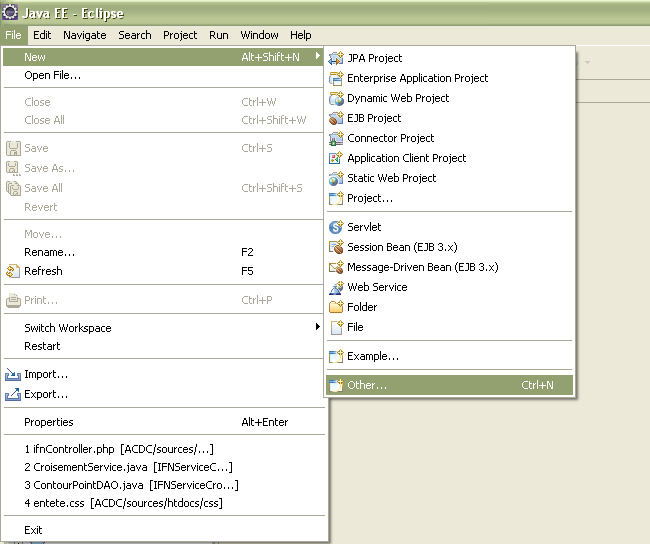
\includegraphics[width=0.39\textwidth]{../../resources/images/guide_installation/geoxygeneEtape1.png}}&
  \imagetop{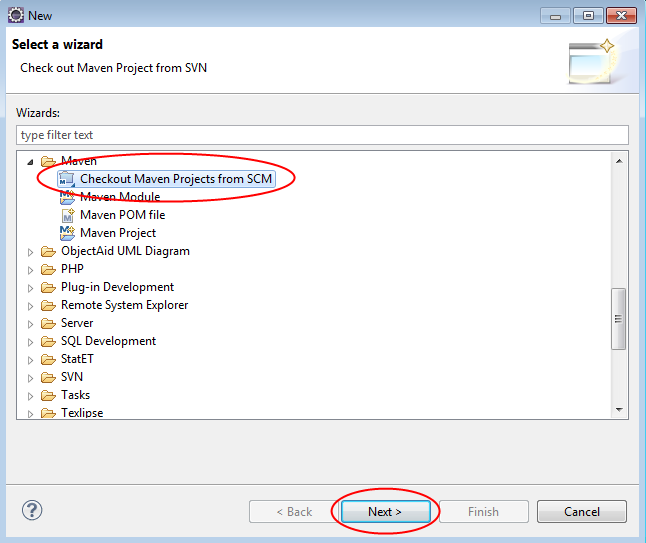
\includegraphics[width=0.61\textwidth]{../../resources/images/guide_installation/geoxygeneEtape2.png}}
\end{tabular}
\end{center}

\newpage

\noindent
Ensuite comme l'indique la figure suivante :

\begin{center}
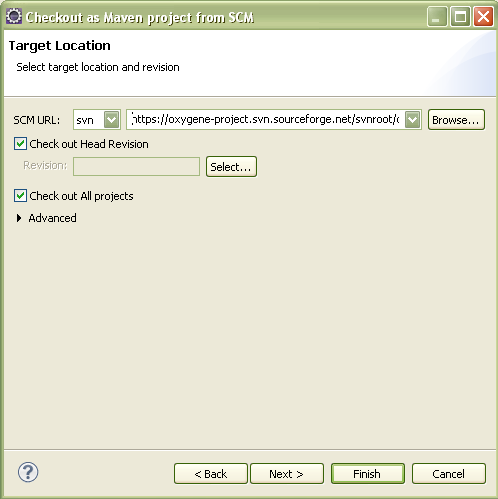
\includegraphics[width=0.5\linewidth]{../../resources/images/guide_installation/geoxygeneEtape3.png}
\end{center}

\noindent
Sélectionner \emph{svn} et indiquer l'adresse du svn de GeOxygene~:\\
\href{https://oxygene-project.svn.sourceforge.net/svnroot/oxygene-project/main/trunk/geoxygene}{https://oxygene-project.svn.sourceforge.net/svnroot/oxygene-project/main/trunk/geoxygene}, 

\bigskip

\noindent
puis cliquer sur "Next".

\bigskip

\noindent
Dans le panneau suivant, vous pouvez:
\begin{itemize}[label=--, leftmargin=* ,parsep=0cm,itemsep=0cm,topsep=0cm]
\item sélectionner le répertoire où sera stocké votre projet (par défaut dans le workspace courant), 
\item ajouter le projet à un working set (c'est à dire un groupe de projets)
\item modifier le nom du (ou des) projet(s) récupéré (s) (dans Advanced). Cette dernière option est utile si vous avez déjà des projets portant des noms identiques ou similaires ou si vous souhaitez ajouter à tous les projets récupérés un préfixe, un suffixe, ou utiliser un template de nom comme [groupId].[artifactId]-[version] qui vous créera, pour geoxygene, un projet nommé \emph{fr.ign.cogit.geoxygene-1.5}.
\end{itemize}

\begin{center}
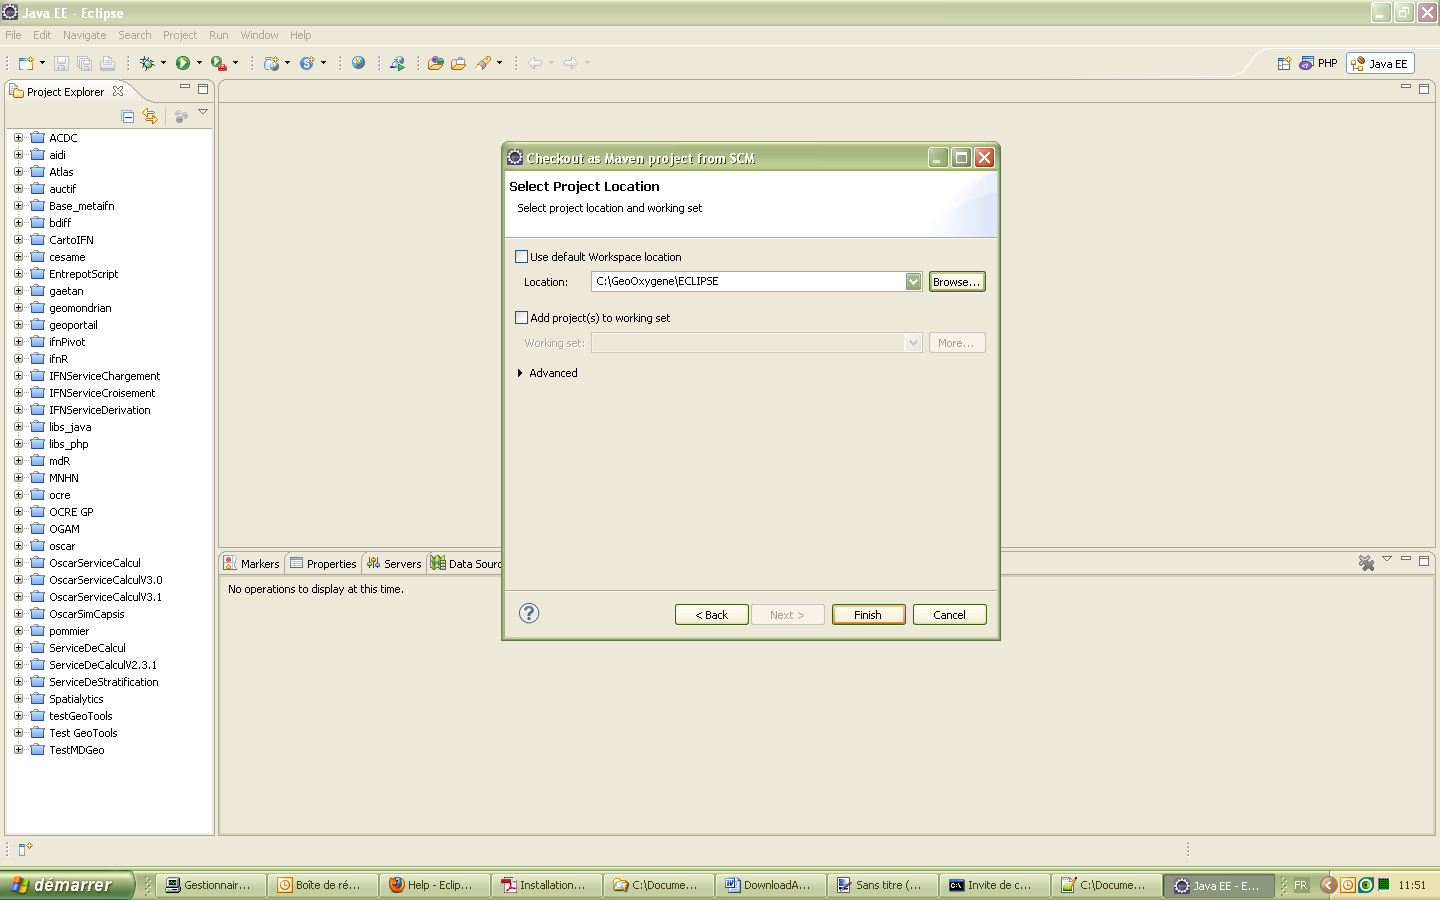
\includegraphics[width=0.5\linewidth]{../../resources/images/guide_installation/geoxygeneEtape4.png}
\end{center}

\bigskip

\noindent
Cliquez ensuite sur Finish.


%---------------------------------------------------------------------------------
\section{Compilation}

Si tout se passe bien, Maven devrait récupérer tous les jars nécessaires et configurer le projet pour la compilation. Si vous utilisez l'option de compilation automatique, vous n'avez rien à faire, sinon, faites un build.

m2eclipse modified the Run As... and Debug As... menus to allow you to run a Maven build within Eclipse. Figure 4.2, “Running
an Eclipse build with Run As..” shows the Run As... menu for an m2eclipse project. From this menu you can run one of the more
common lifecycle phases like clean, install, or package. You can also load up the Run configuration dialog window and configure
a Maven build with parameters and more options.




%---------------------------------------------------------------------------------
\section{Exécution des exemples}
Une application exemple peut \^etre exécutée~: \emph{fr.ign.cogit.geoxygene.appli.GeOxygeneApplication}.


\section{Configuration}

\begin{itemize}[leftmargin=* ,parsep=0cm,itemsep=0cm,topsep=0cm]
\item Activation de la console Maven.

Ouvrer la fenêtre de la console en cliquant sur : {\emph{Window} $\Rightarrow$ \emph{Show View}  $\Rightarrow$ \emph{Console}}. Puis cliquer sur la petite flèche complètement à droite de la fenêtre "Open Console" et sélectionner "Maven Console" comme indiqué ci-dessous :

\begin{center}
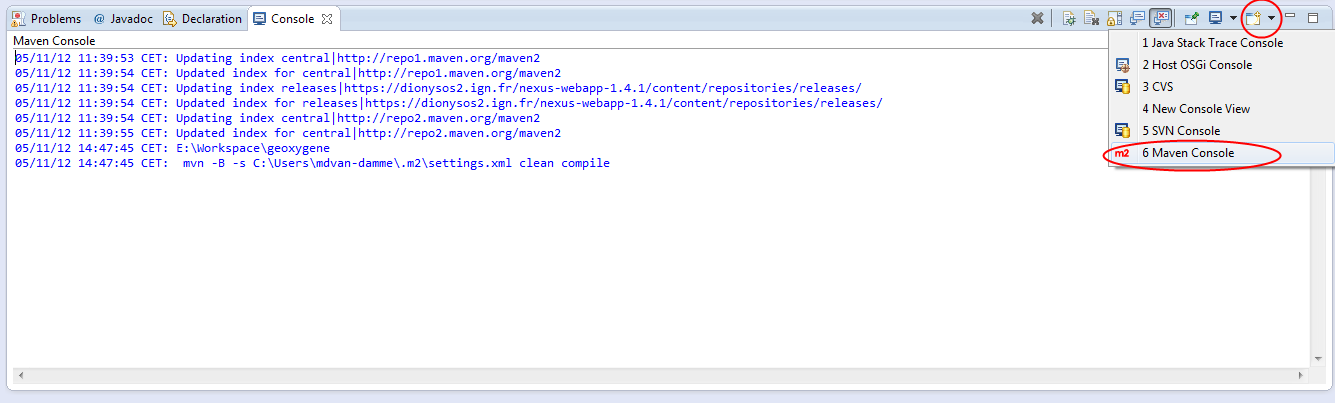
\includegraphics[width=0.5\linewidth]{../../resources/images/guide_installation/geoxygeneEtape5.png}
\end{center}

Il peut être utile de travailler avec la sortie de débogage Maven pour diagnostiquer les problèmes.


\end{itemize}


\begin{itemize}[leftmargin=* ,parsep=0cm,itemsep=0cm,topsep=0cm]
\item convention de codage
\item accès aux bases de données
\item journalisation
\item encodage
\end{itemize}
